\documentclass{gescons}

\genre {Entrevista}
\author{Victor Bolfe}
\title{Estado Vibracional: 100 Perguntas e~Respostas}
\paginaurl{https://www.youtube.com/live/vIFaWEb3UeI}

\begin{document}
    \makeentrevistatitle
    \coverart{back/Victor_Bolfe}

    \begin{multicols}{2}


\begin{center}
    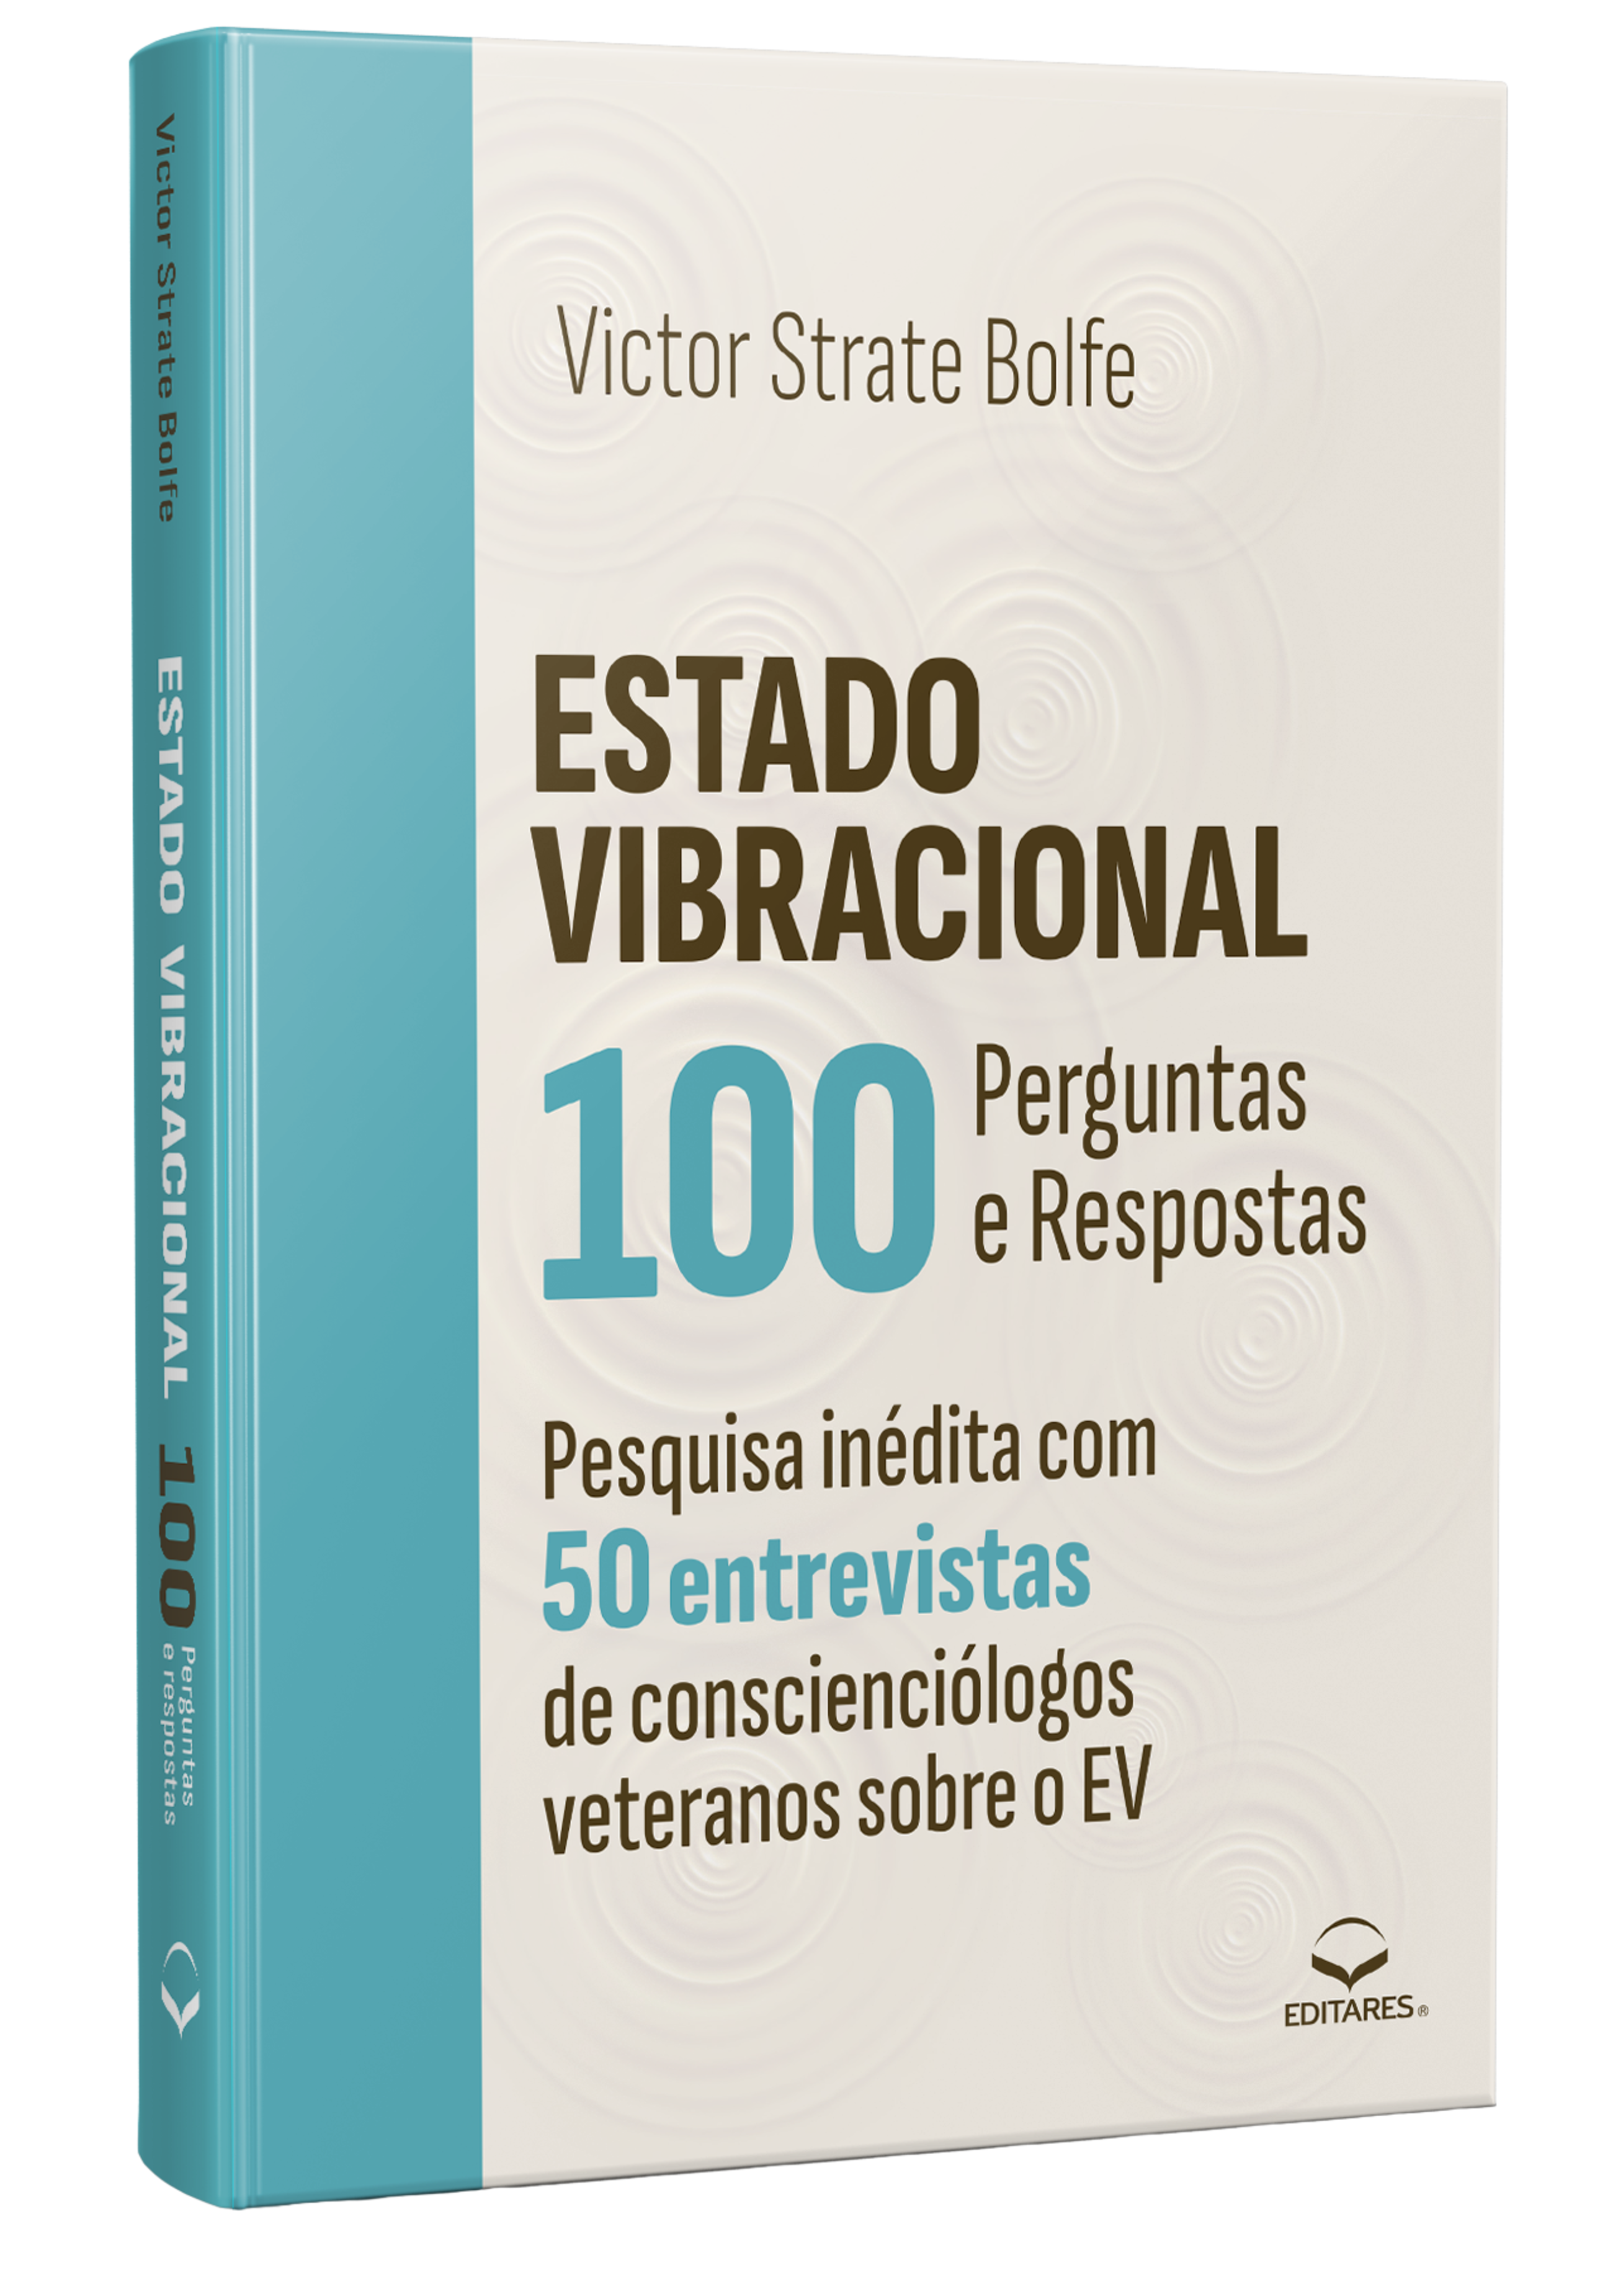
\includegraphics[width=8cm]{articles/entrevista/mockups/Victor-Bolfe}
\end{center}

\textbf{1. Qual foi a~motivação para a~escrita da obra? Por que a~definição deste tema para publicação de um livro?}

Aprofundar a~pesquisa do EV de modo técnico, didático, detalhista, científico, profundo e~exaustivo, deixando legado assistencial substancial para a~humanidade. 

O tema foi definido por consolidar uma década de desenvolvimento da especialidade de pesquisa do autor sobre o~Estado Vibracional. 

\textbf{2. Quais foram as principais percepções, intra e~extrafísicas, durante a~pesquisa e~a~escrita da obra? E~posterior ao lançamento?}

O EV é~tema básico nos estudos da Conscienciologia, porém ainda demanda muito esclarecimento e~teática. Existe muito incentivo dos amparadores para a~qualificação do EV por parte dos participantes da CCCI. 

\begin{pullquote}
    ``Existe muito incentivo dos amparadores para a~qualificação do EV por parte dos participantes da CCCI.''
\end{pullquote}


\textbf{3. Qual o~maior aprendizado com a~escrita desta obra?}

Uma obra incialmente simples pode tomar grandes proporções caso o~autor esteja aberto ao processo. 

\textbf{4. O~que poderia dizer como incentivo para que mais pesquisadores invistam na publicação de obras conscienciológicas?}

A publicação de livro conscienciológico é~oportunidade para materializar legado tarístico perpétuo, resultando em dividendos cármicos exponenciais ao longo do périplo evolutivo.

\begin{pullquote}
    ``A publicação de livro conscienciológico é~oportunidade para materializar legado tarístico perpétuo.''
\end{pullquote}


    
    \end{multicols}
\end{document}
